\documentclass{beamer}
\usepackage{amsfonts, amsmath, graphicx, verbatim}
\usetheme{Warsaw}

\title[NZSA 2011 Conference]{\bf SNM-GARCH: \\
       A Semi-Parametric Mixture Model}
\author[]{\em  Supervisor: Dr Yong Wang\\ Michael Kao}
\institute{Dept. of Statistics, University of Auckland}
\date{}

\begin{document}

\begin{frame}
\titlepage
\end{frame}

\frame{
  \frametitle{Outline}
  \tableofcontents
}

\section{Introduction}
\frame{
   \frametitle{History}
   \begin{itemize}
   \item The introduction of ARCH/GARCH by Engle(1982) and
     Bollerslev(1986), made major contribution to the advancement of
     volatility modelling.
   \item A paper by Tim Bollerslev (2008) documented more than 100
     generalisation/extension of the ARCH/GARCH type model.
   \item Its great, but we can do better!
   \end{itemize}
}
\frame{
   \frametitle{Motivation}
   \begin{itemize}
   \item Problem: The standard normal assumption is often violated in
     practice due to the skewness and the heavy-tail nature of the
     financial data.
   \item Solution: Relax the standard normal assumption to a Scale
     Normal Mixture (SNM).
   \item Result: Improved fit and decomposition of  the source
     of volatility.
   \end{itemize}
}

\section{Background}
\subsection{GARCH}
\frame{
   \frametitle{The general GARCH(p, q) model}
   The GARCH model proposed by Tim Bollerslev (1986).
   \begin{block}{GARCH(p, q)}
   \begin{align*}
     x_t &= \mu + \sigma_t \epsilon_t \;\;\;\;\;\;\;\;\;\;\;
            \epsilon_t \sim N(0, 1)\\
     \sigma_t^2 &= \alpha_0 + \sum_{i = 1}^p \beta_i \sigma_{t-i}^2 +
      \sum_{j = 1}^q \alpha_j x_{t-j}^2\\
   \end{align*}
   \end{block}
   Where the log return $x_t$ is defined as $\nabla \log(P_t)$.
}

\subsection{Semi-Parametric Mixture Model}
\frame{
\frametitle{Semi-Parametric Mixture Model}
   \begin{itemize}
    \item Non-parametric $\leftarrow$ Semi-parametric $\rightarrow$
      Parametric.
    \item In this context, the SNM-GARCH model compose of
      parametric estimation of volatility movement and non-parametric
      estimation of the Scale Nomal Mixture (SNM) error distribution.
   \end{itemize}
}

\subsection{The Scale Normal Mixture Distribution (SNM)}
\frame{
    \frametitle{Scale Normal Mixture Distribution}
    A scale normal mixture in its simplest term is just a distribution
    consists of a mixture of normal distributions.
   \begin{block}{Scale Normal Mixture Distribution}
   $$
   \mathnormal{f}(x; G) = \int_{\Omega} \phi(x; \theta) \mathrm{d}G(\theta)
   $$
   \end{block}
   where the $\phi (x; \theta)$ is the Normal component density and
   $G(\theta)$ the mixing distribution function.
}

\frame{
    \frametitle{Scale Normal Mixture Distribution Cont.}
   Since our estimation is based on maximum likelihood with finite data
   points, the MLE of $G(\theta)$ must be discrete and we can rewrite the
   density as the following:
   \begin{block}{Scale Normal Mixture Distribution}
   \begin{align*}
   G(\theta) &= \sum_{i = 1}^m \pi_i \delta_{\theta_i} \\
   \mathnormal{f}(x; \mu, \boldsymbol{\pi}, \boldsymbol{\theta}) &=
             \sum_{i = 1}^m \pi_i \; \phi(\mu, \theta_i),
   \end{align*}
   \end{block}
   Where $\theta_i$'s are the support points of the mixing
   distribution.
}

\section{SNM-GARCH}
\subsection{Model}
\frame{
   \frametitle{Scale Normal Mixture GARCH (p, q)}
   A SNM-GARCH model is simply a GARCH model where
   the assumption of standard normal error distribution is replaced
   with a scale normal mixture (SNM) distribution.
    \begin{block}{SNM-GARCH}
    \begin{align*}
     x_t &= \mu + \sigma_t \epsilon_t \;\;\;\;\;\;\;\;\;\;\;
            \epsilon_t \sim SNM(0, G)\\
     \sigma_t^2 &= \alpha_0 + \sum_{i = 1}^p \beta_i \sigma_{t-i}^2 +
      \sum_{j = 1}^q \alpha_j x_{t-j}^2\\
     \end{align*}
     \end{block}
}

\subsection{Estimation}
\frame{
    \frametitle{Estimation}
     The estimation is carried out under the semi-parametric mixture
     framework in Wang (2010) via maximum likelihood estimation.\\
     \begin{block}{CNM-MS algorithm}
     \begin{enumerate}
     \item Add support point via the CNM algorithm.
     \item Use BFGS to optimise the likelihood with respect to all
       the parameters ($\alpha_0, \alpha_1, \beta_1, \mu,
       \boldsymbol{\pi}, \boldsymbol{\theta}$) and update.

     \item Scale to ensure the Scale Normal Mixture Distribution has
       variance 1.
     \end{enumerate}
     \end{block}
}
\frame{
    \frametitle{Likelihood Function}
    \begin{block}{Likelihood Function}
     \begin{align*}
     &\mathnormal{l}(x; \alpha_0, \alpha_1, \beta_1, \mu, \sigma_t,
     \boldsymbol{\theta})\\
     =&\prod_{t = 1}^T
     \prod_{i=1}^m \frac{1}{\sqrt{2 \pi \theta_i^2 (\alpha_0 +
     \sum_{i=1}^p \alpha_1 \sigma_{t-1}^2 + \sum_{j = 1}^q \beta_1
     x_{t-1}^2)}} \\
     &\exp
       \left(\frac{-(x_t - \mu)^2}{2 \theta_i^2 (\alpha_0 + \sum_{i = 1}^p
     \alpha_1 \sigma_{t-1}^2 + \sum_{j = 1}^q \beta_1
     x_{t-1}^2)}\right),\\
     &\alpha_0 > 0, \forall \alpha_i \ge 0, \forall \beta_i \ge 0
     \end{align*}
     \end{block}
}


\section{Examples}
\subsection{New York Stock Exchange}
\frame{
   \frametitle{NYSE}
   This example is taken from Shumway and Stoffer (2010). The data
   consists of 2000 daily log return of the New York Stock Exchange time
   series over the period starting from February 1st, 1984 and ends on
   the December 31st, 1991.
}


\frame{
    \frametitle{NYSE}
    \begin{figure}
    \centering
    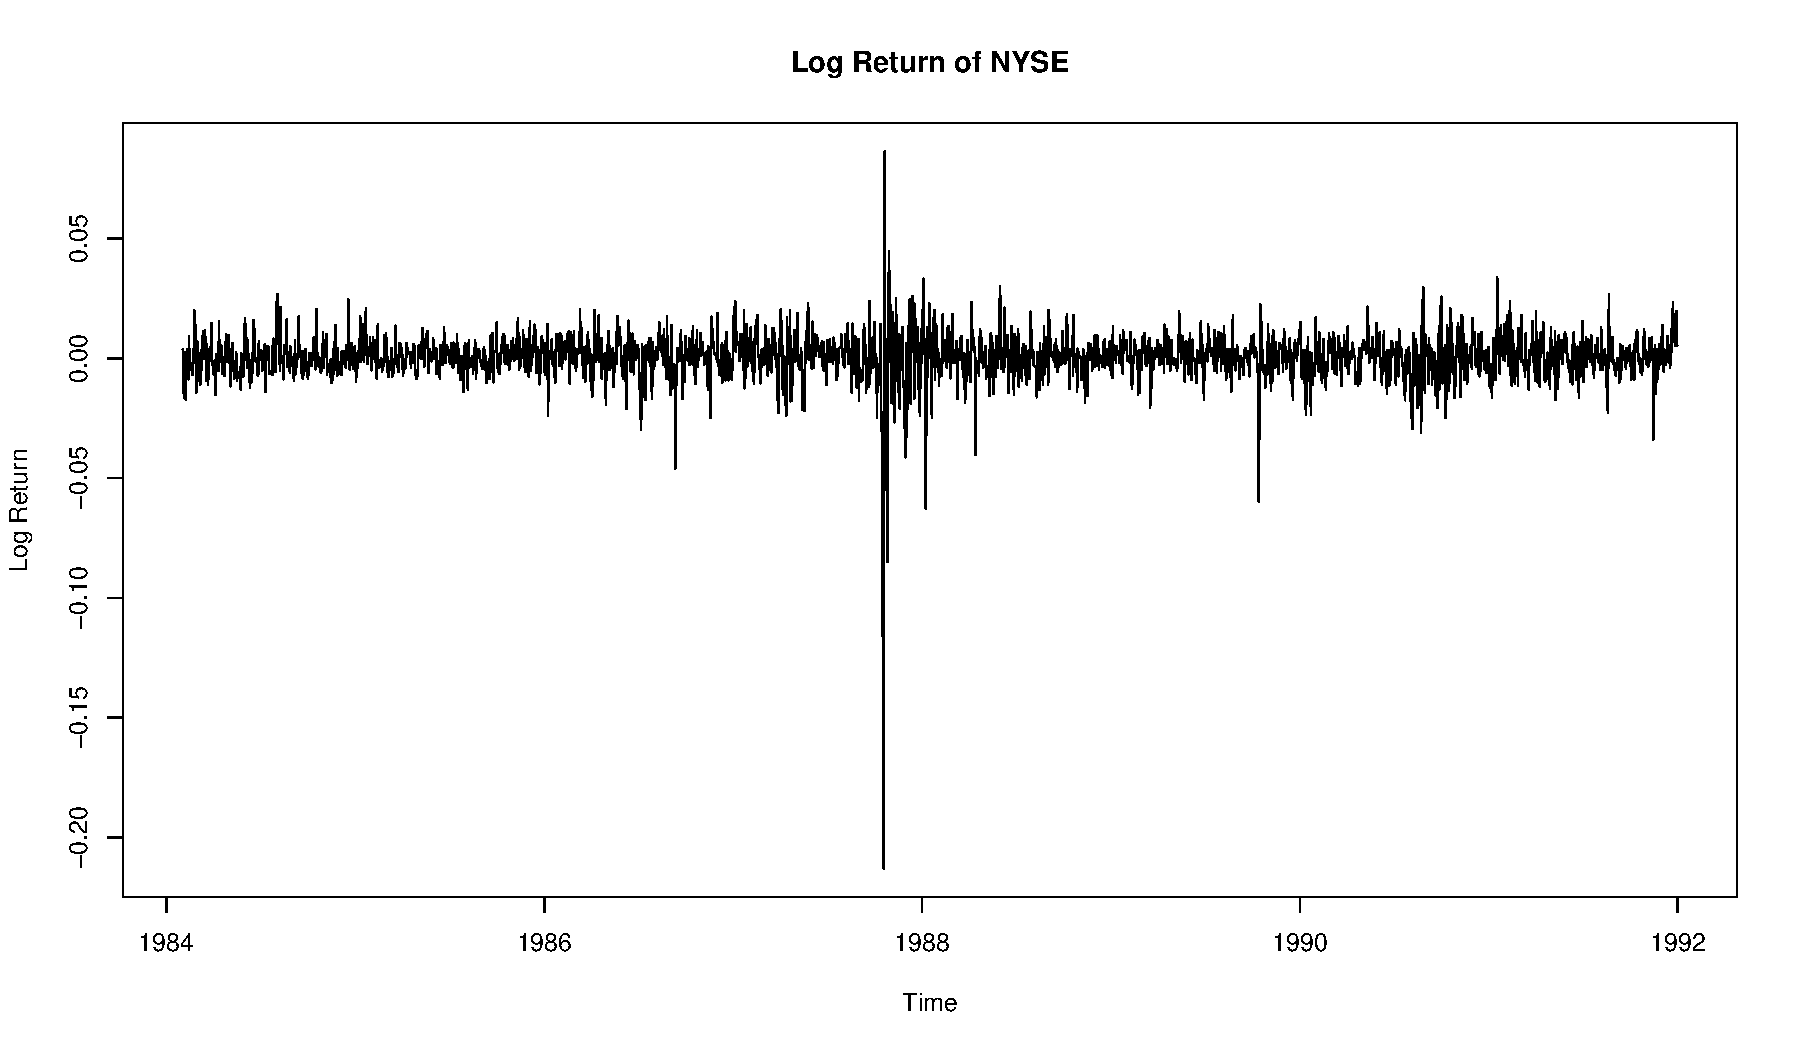
\includegraphics[width = 10cm, height = 5cm]{nyse.pdf}
    \caption{The plot of the daily log return. The large negative
      spike corresponds to the market crash on October 19th, 1987 also
      known as the Black Monday}
    \end{figure}
}

\frame{
    \frametitle{Fit}
    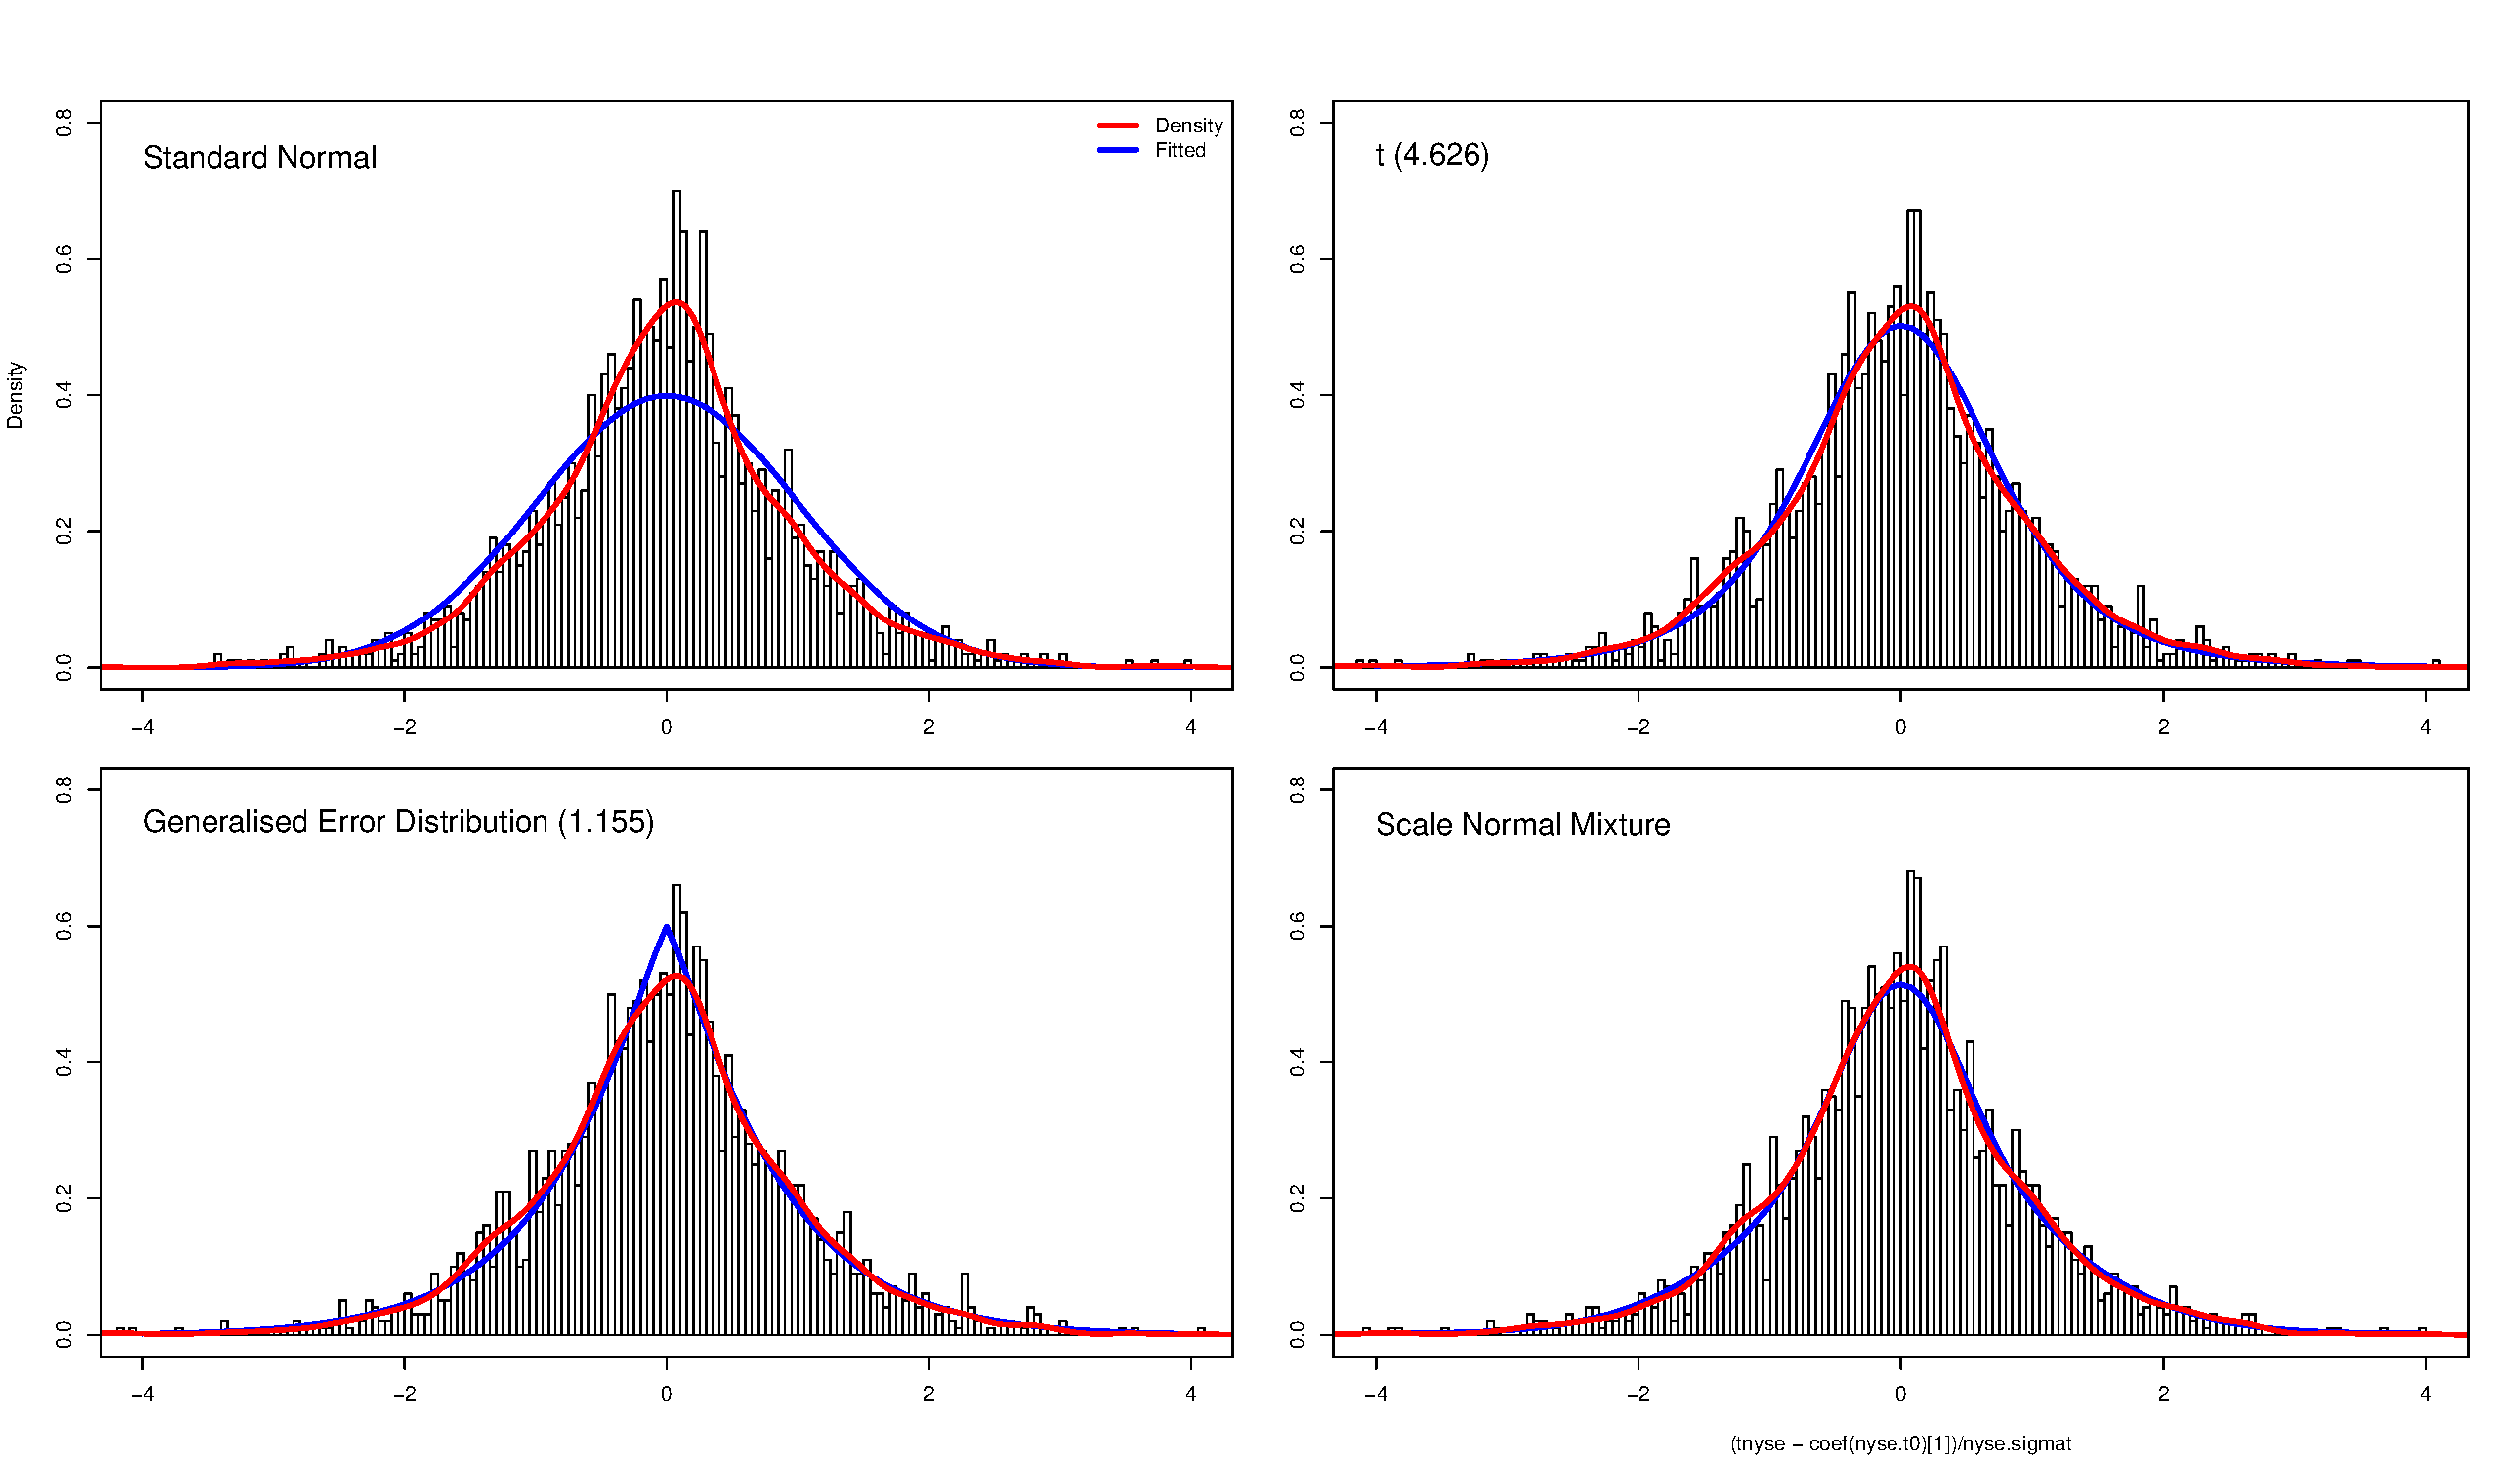
\includegraphics[scale = 0.25]{nyseErrorDistAll.pdf}
}

\frame{
    \frametitle{Zoomed Fit}
    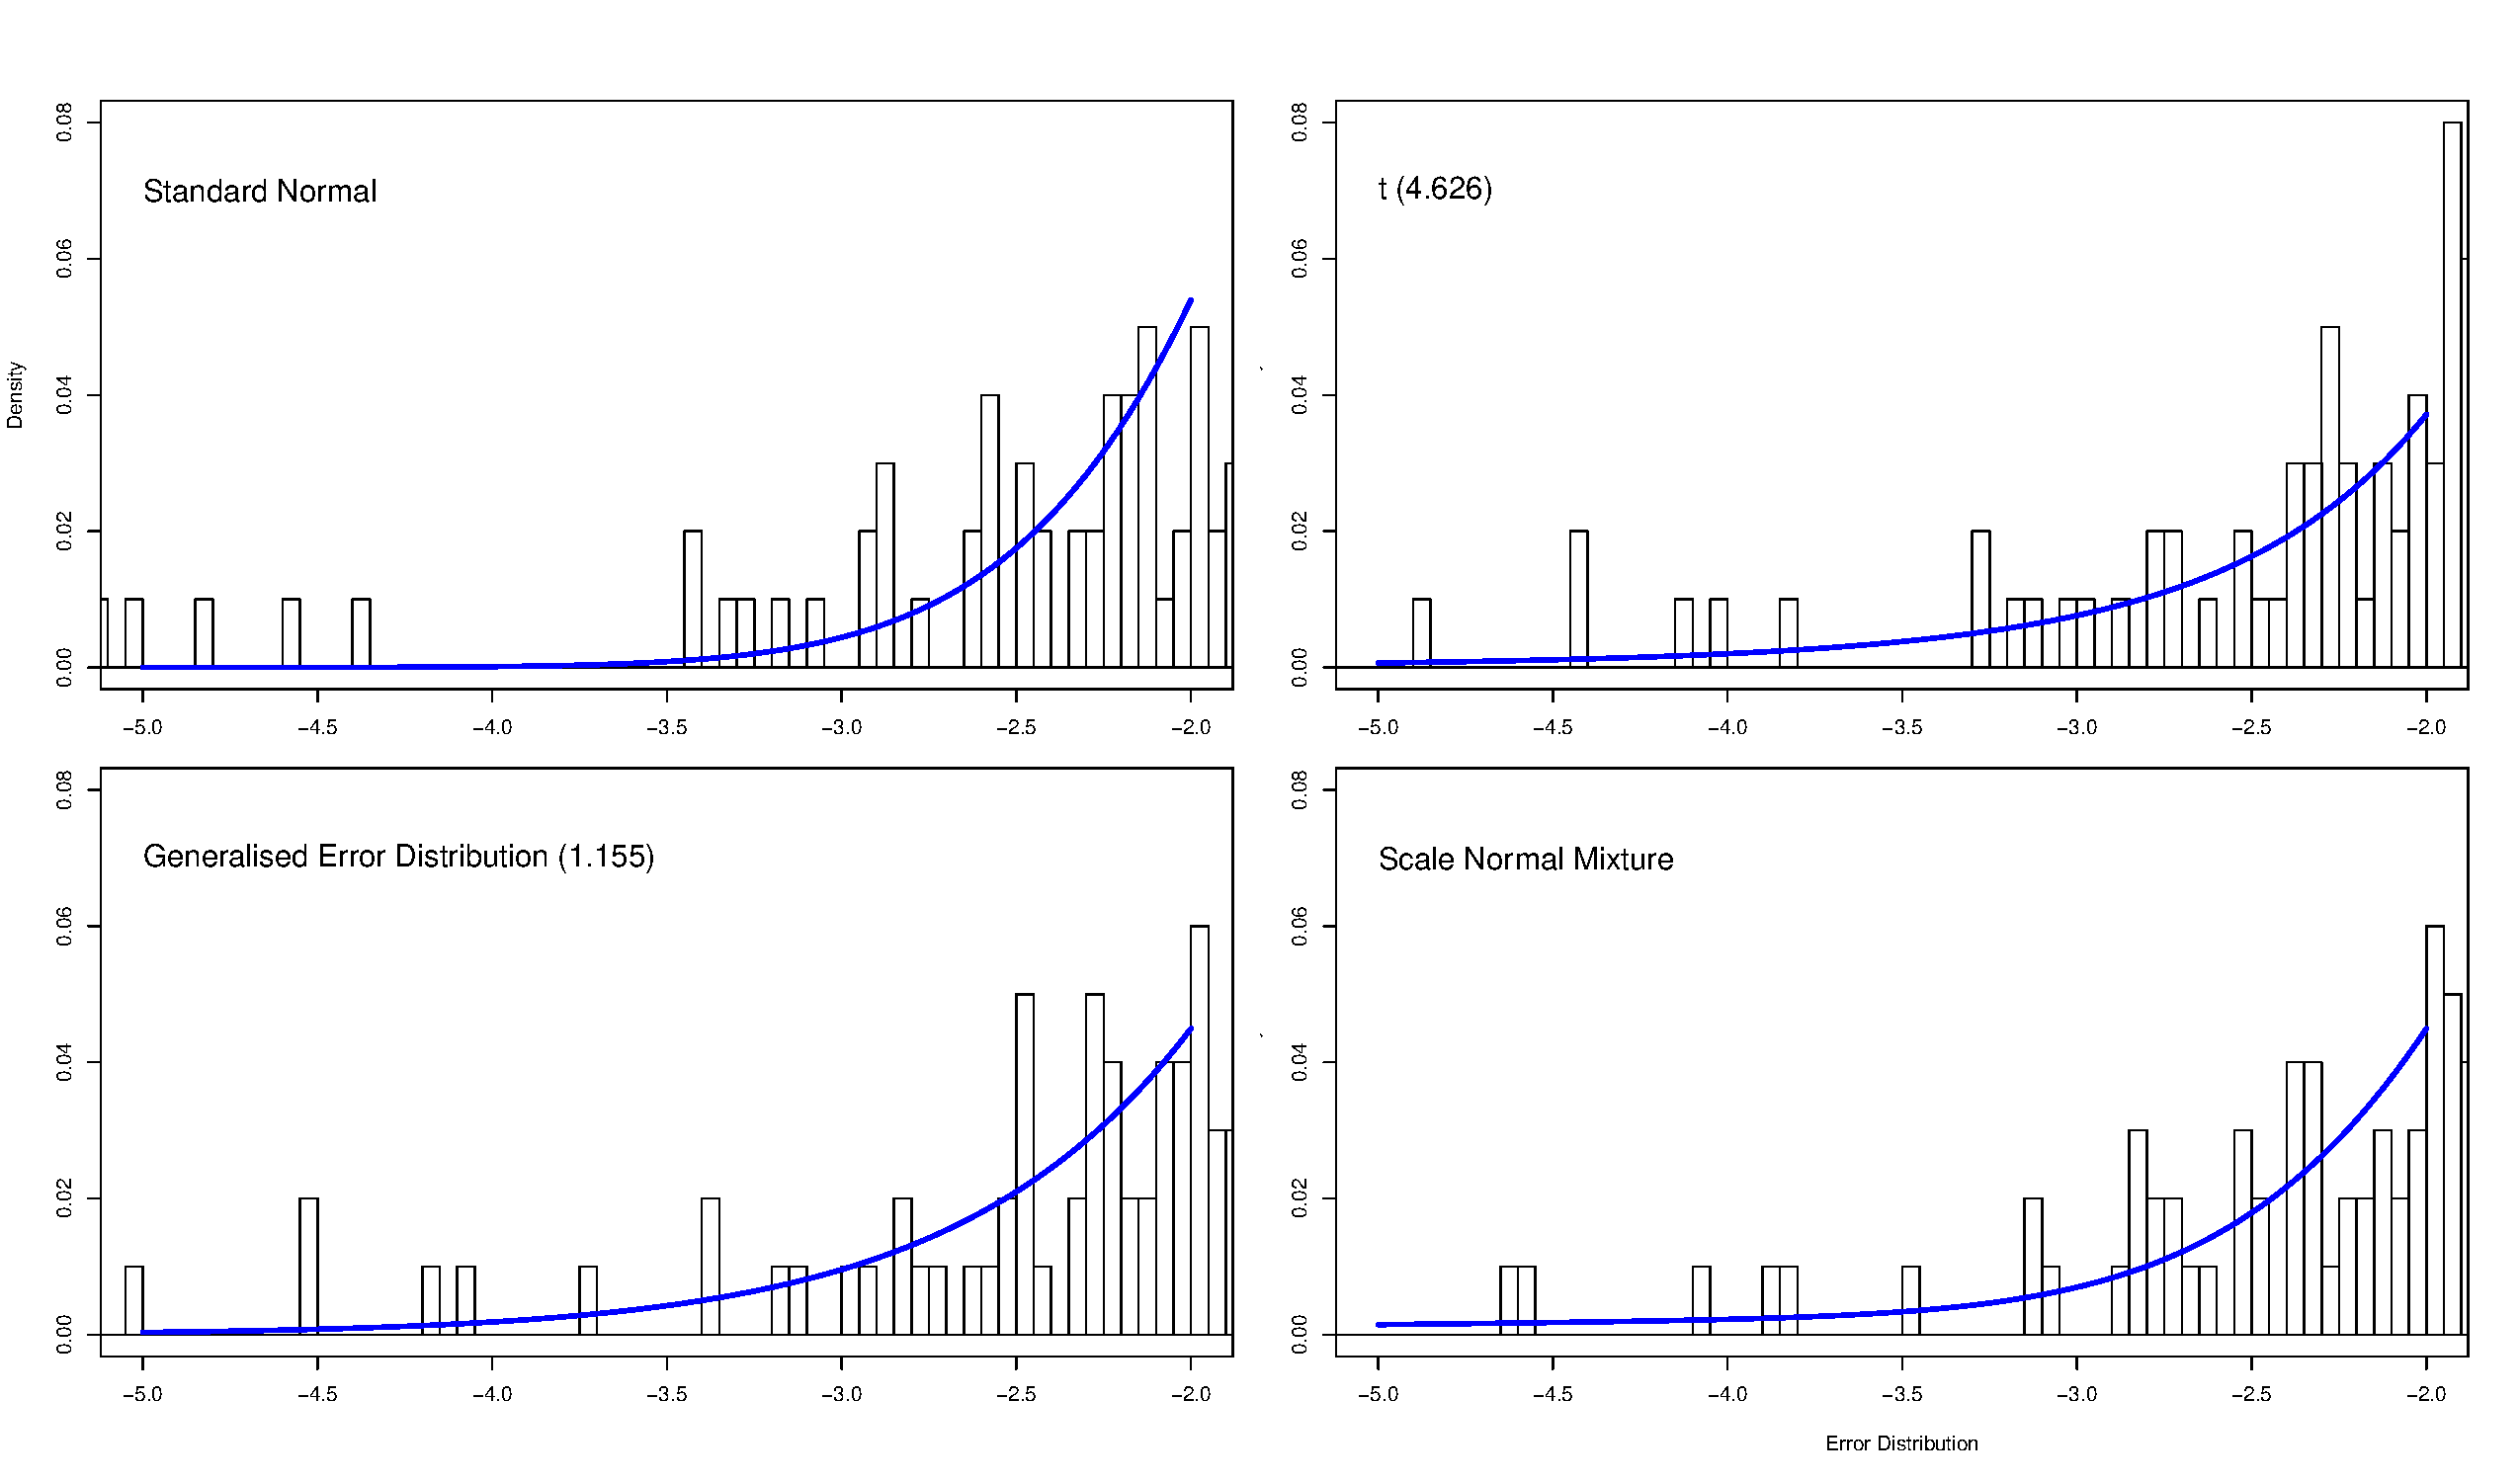
\includegraphics[scale = 0.25]{nyseErrorDistZoomLow.pdf}
}


\subsection{Standard \& Poor 500}
\frame{
   \frametitle{S\&P 500}
   This dataset contains the daily log return of the S\&P 500 since
   Janurary 1st, 2005 to current date.
}


\frame{
    \frametitle{S\&P 500}
    \begin{figure}
    \centering
    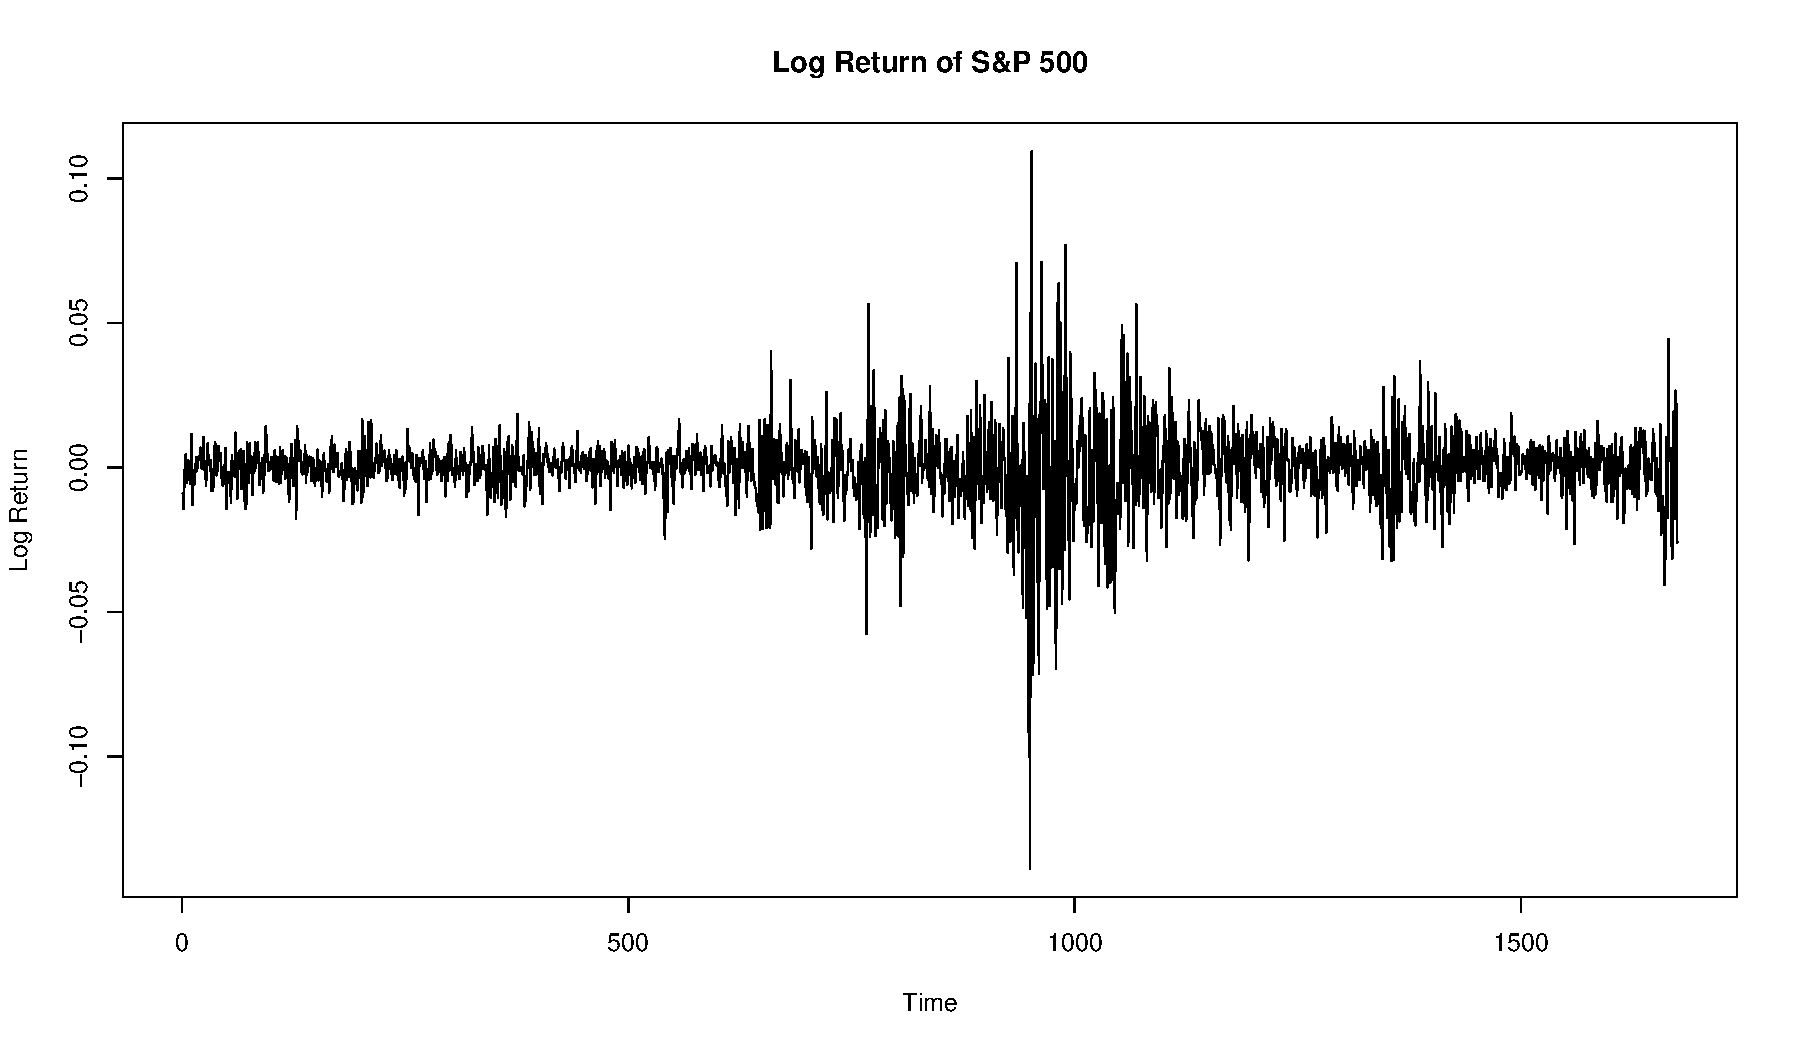
\includegraphics[width = 10cm, height = 5cm]{sp.pdf}
    \caption{The S\&P 500 data, we can see the volatility structure is
    quite different to that of the NYSE.}
    \end{figure}
}

\frame{
    \frametitle{Fit}
    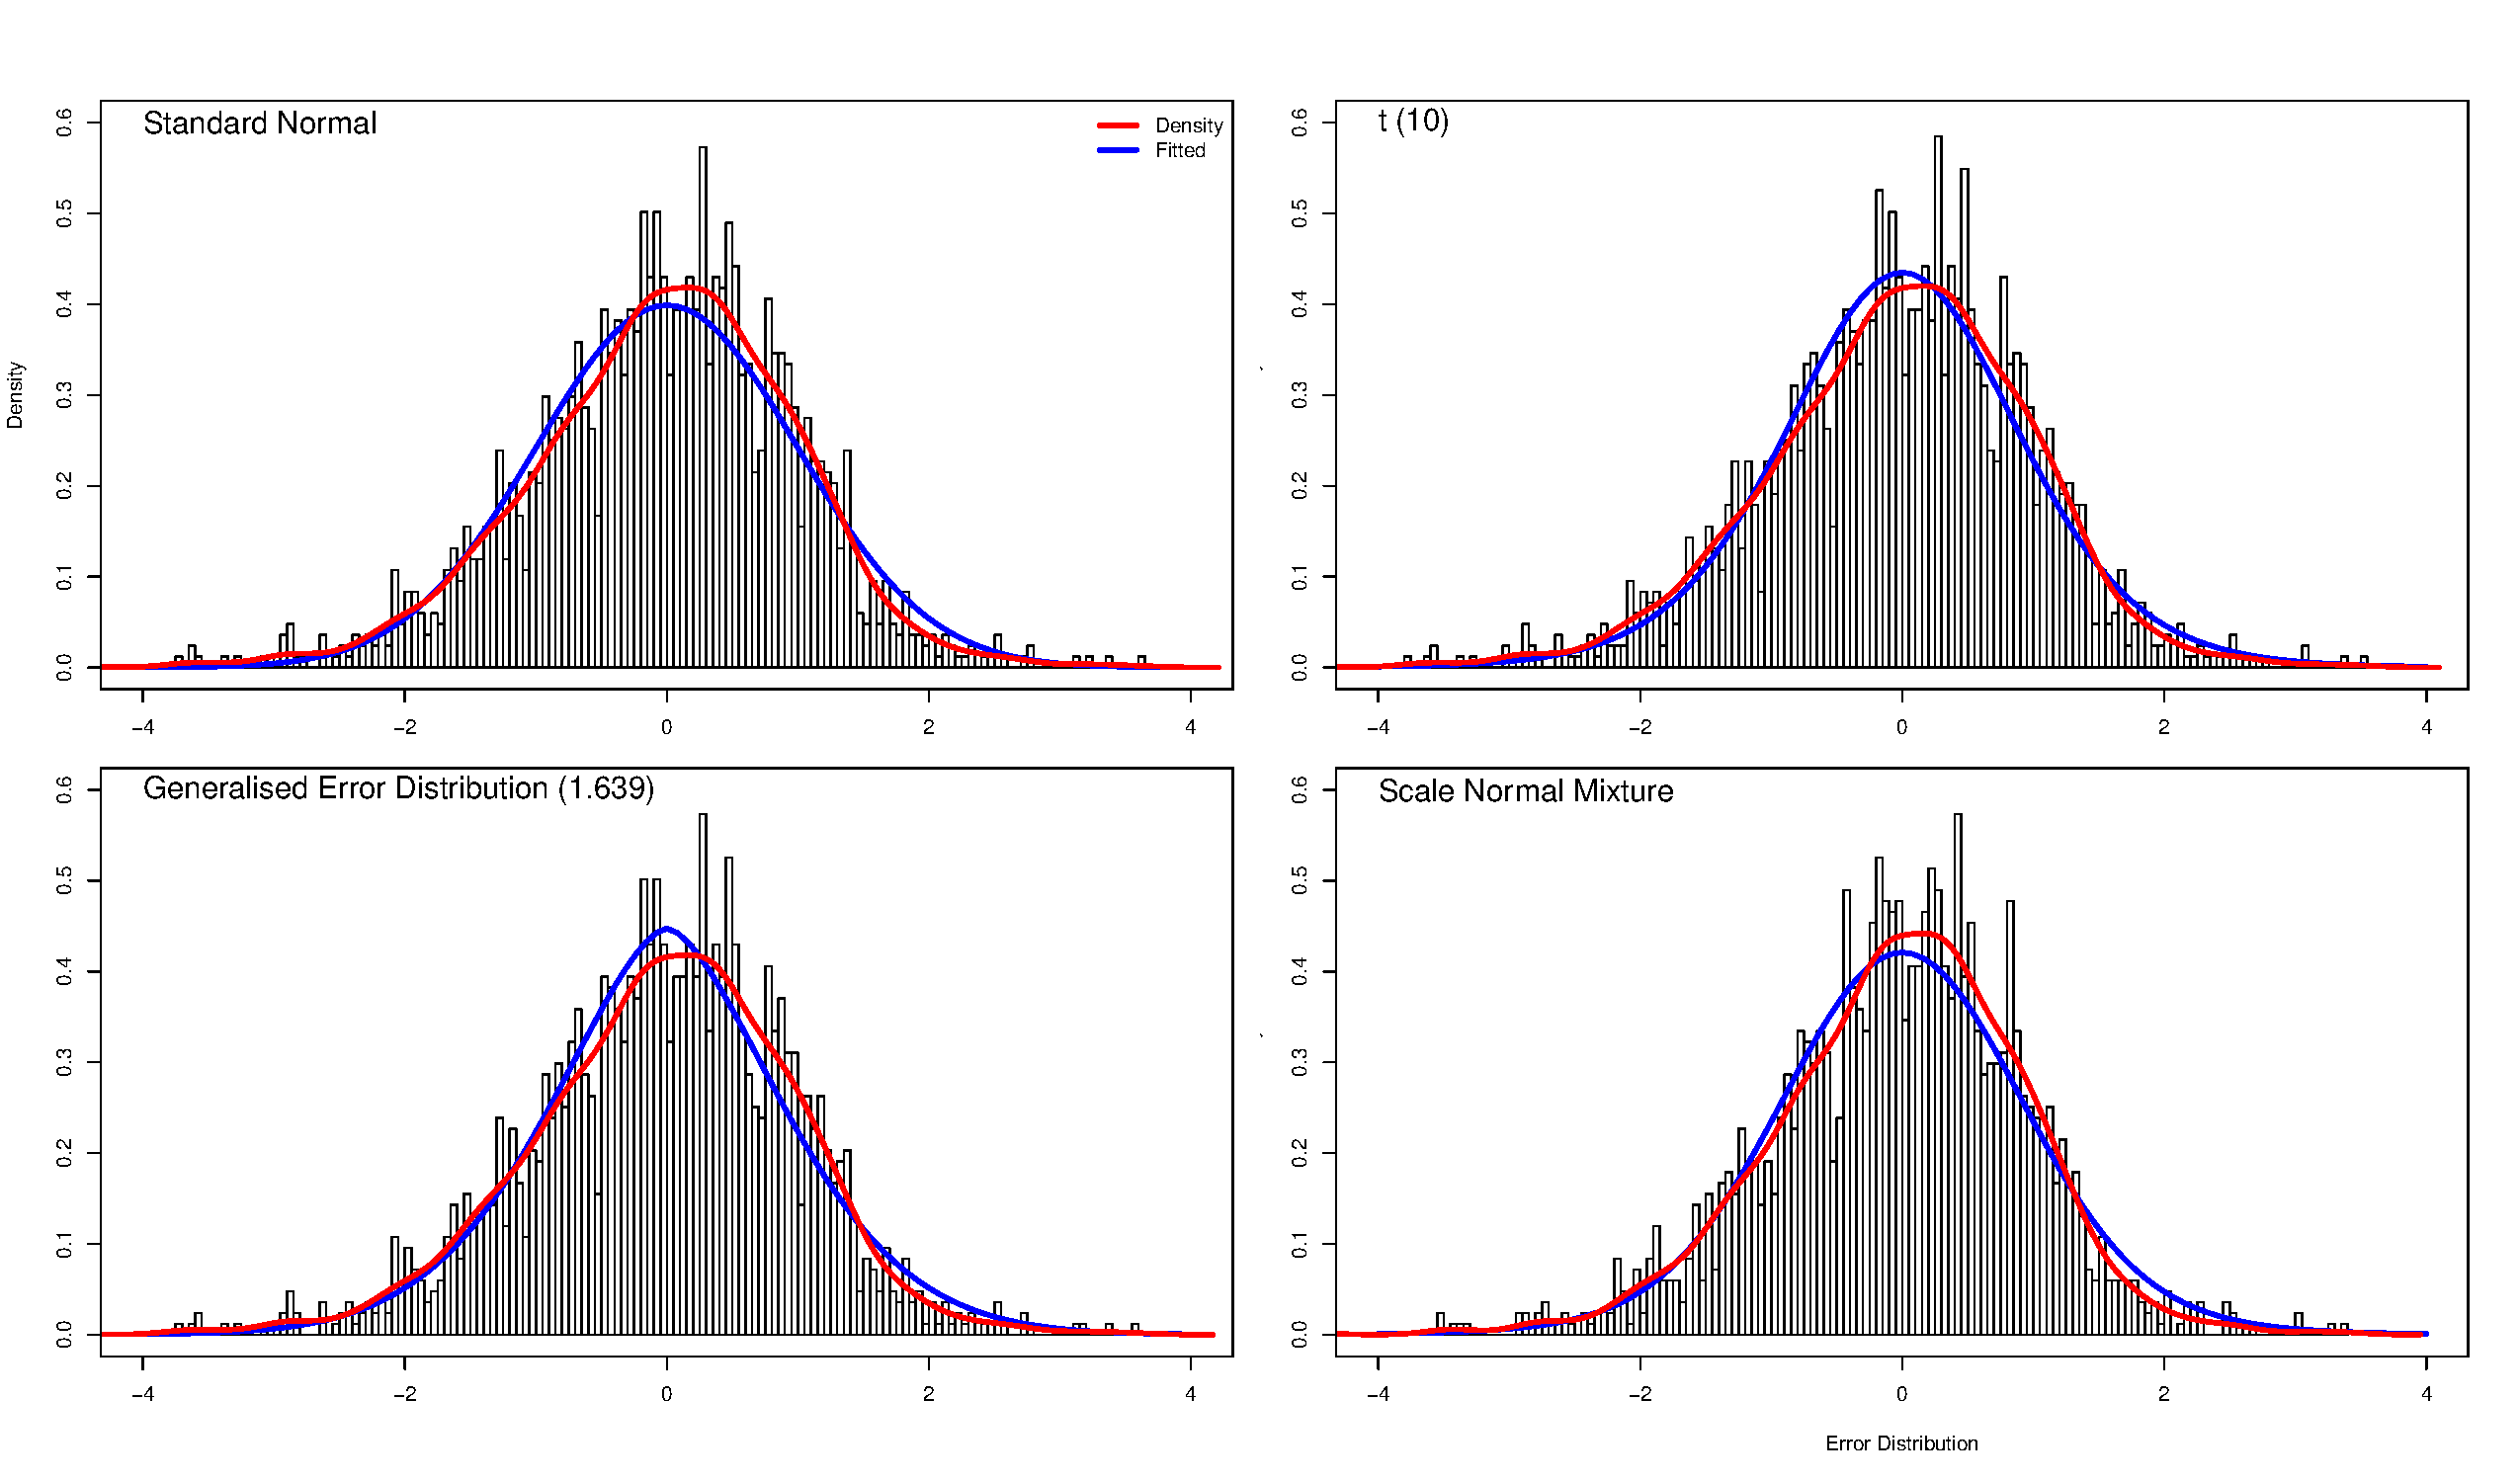
\includegraphics[scale = 0.25]{spErrorDistAll.pdf}
}

\frame{
    \frametitle{Fit Zoomed}
    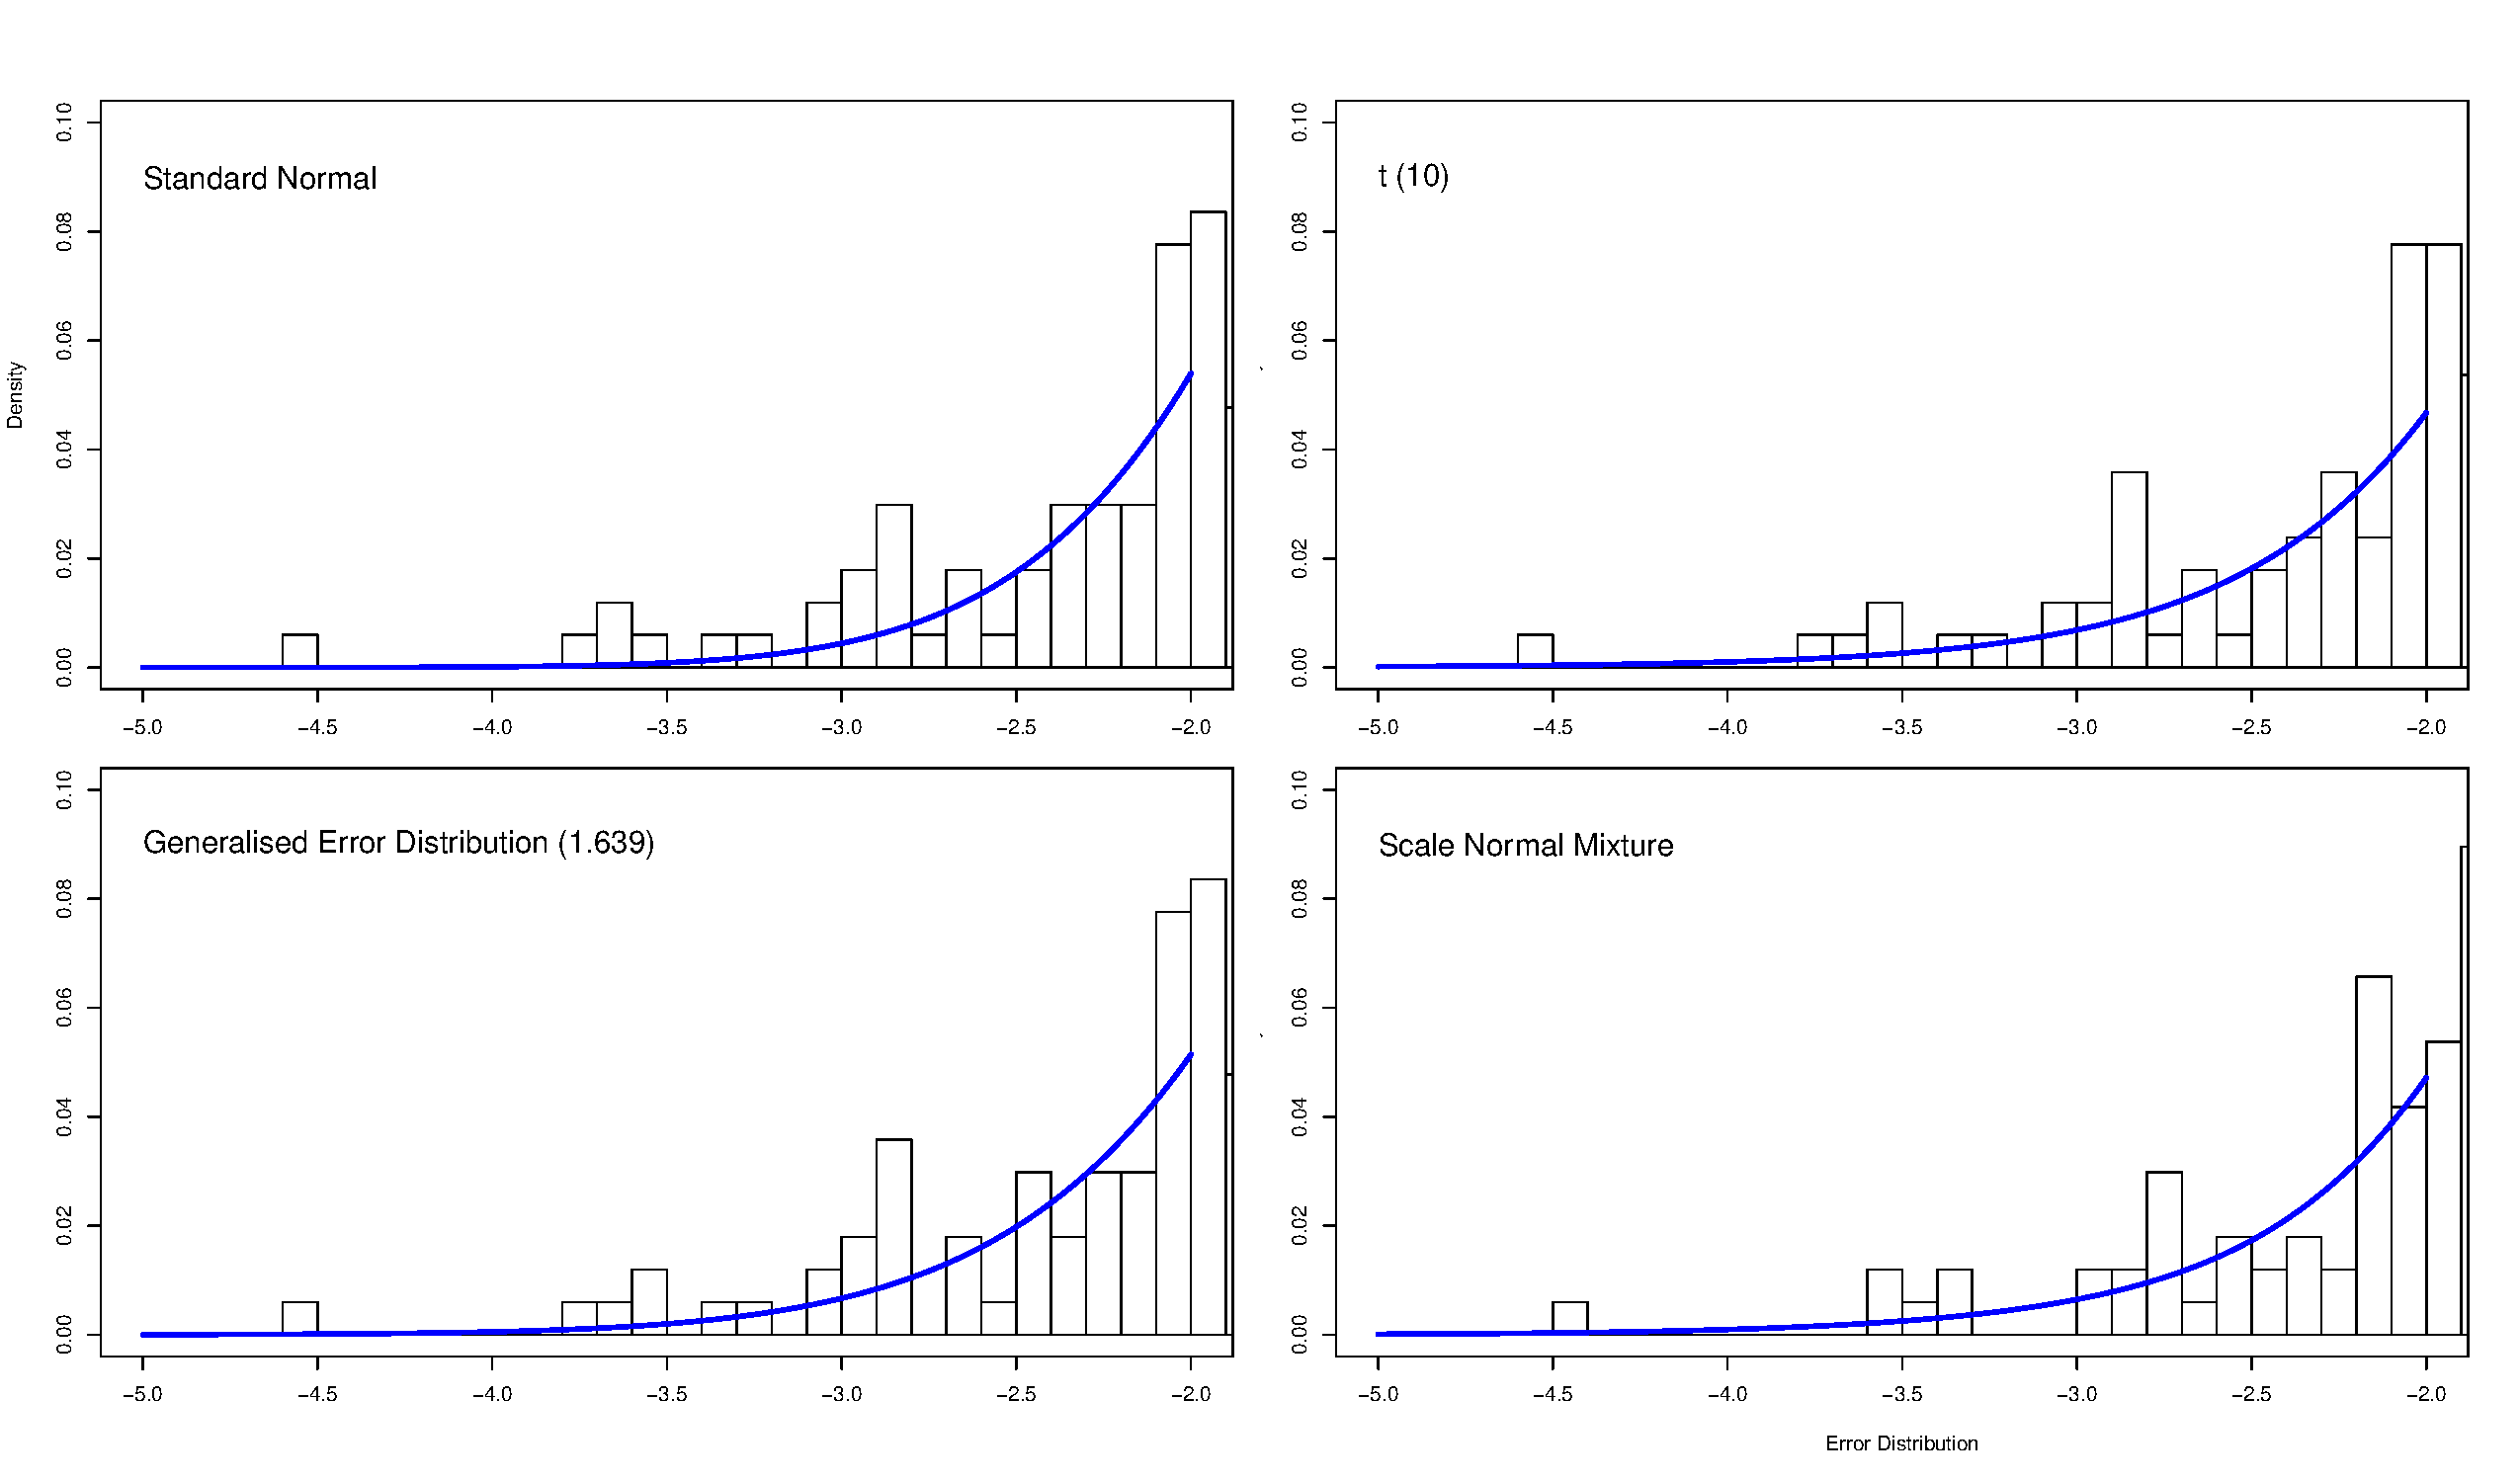
\includegraphics[scale = 0.25]{spErrorDistZoomLow.pdf}
}

\section{Understand the source of volatility}
\frame{
    \frametitle{NYSE}
    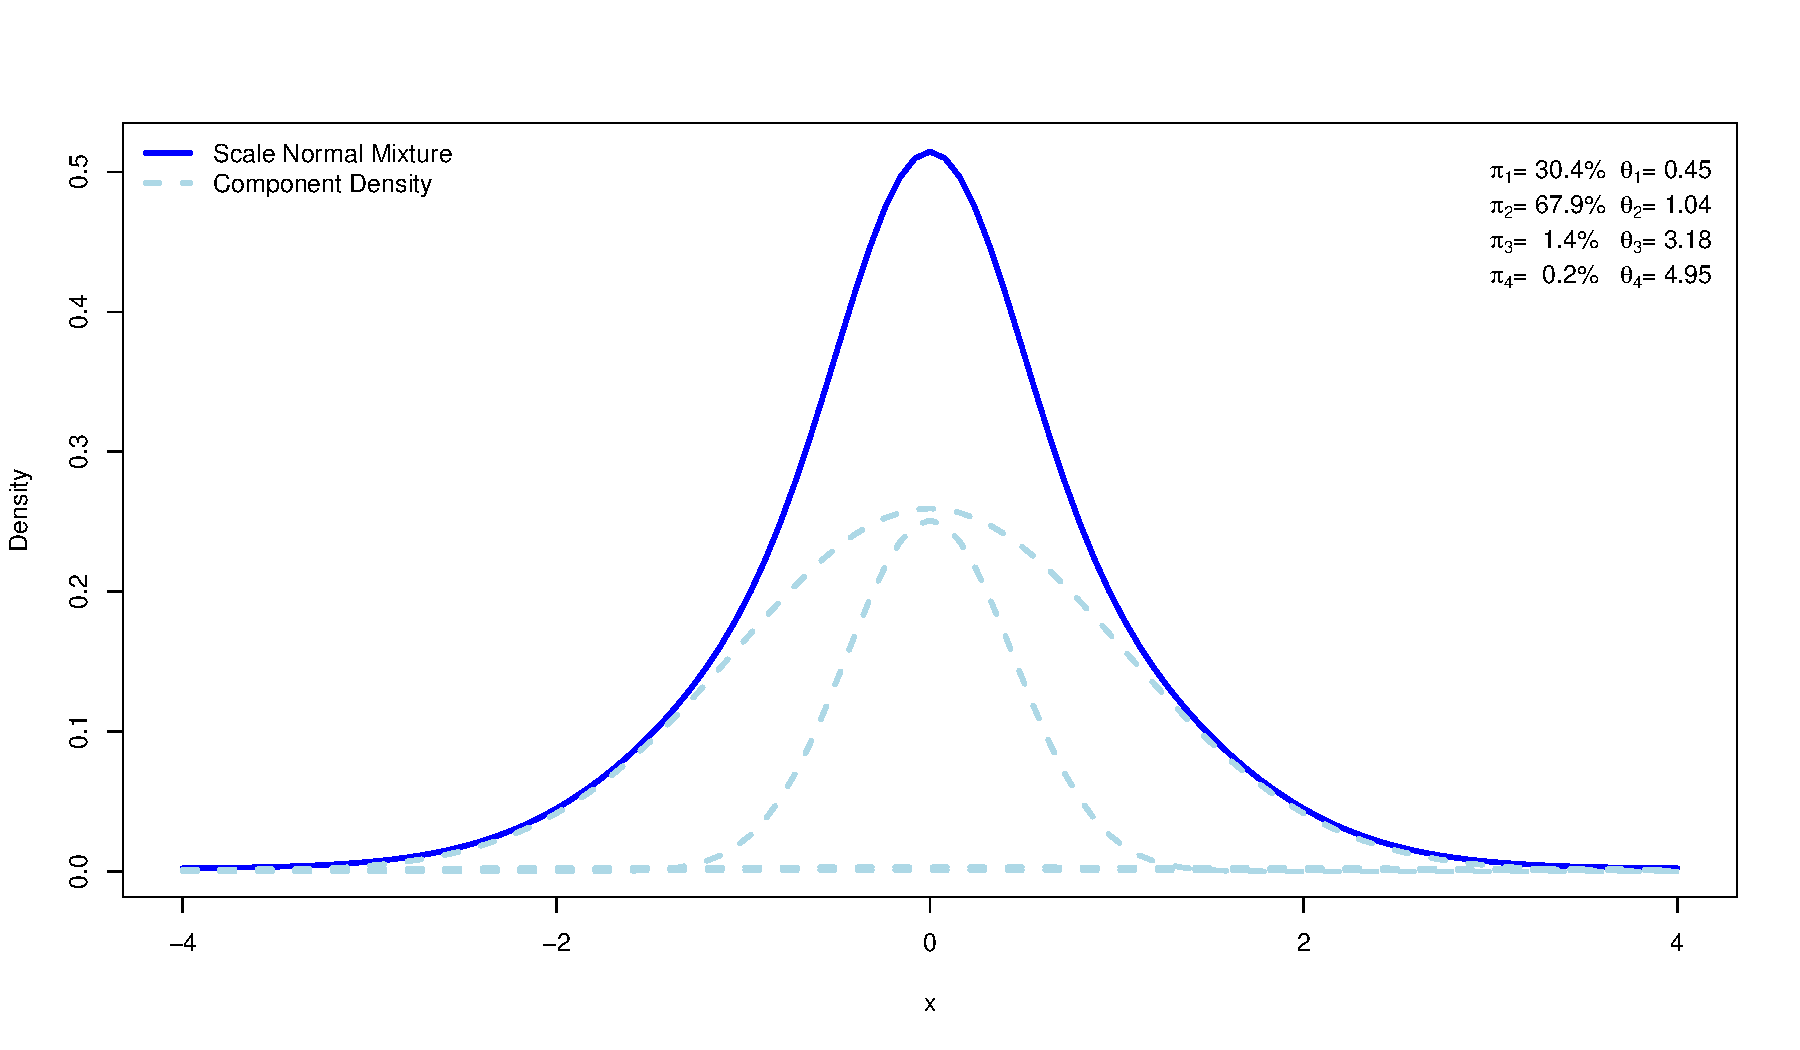
\includegraphics[scale = 0.35]{nyseComp.pdf}
}

\frame{
    \frametitle{S\&P 500}
    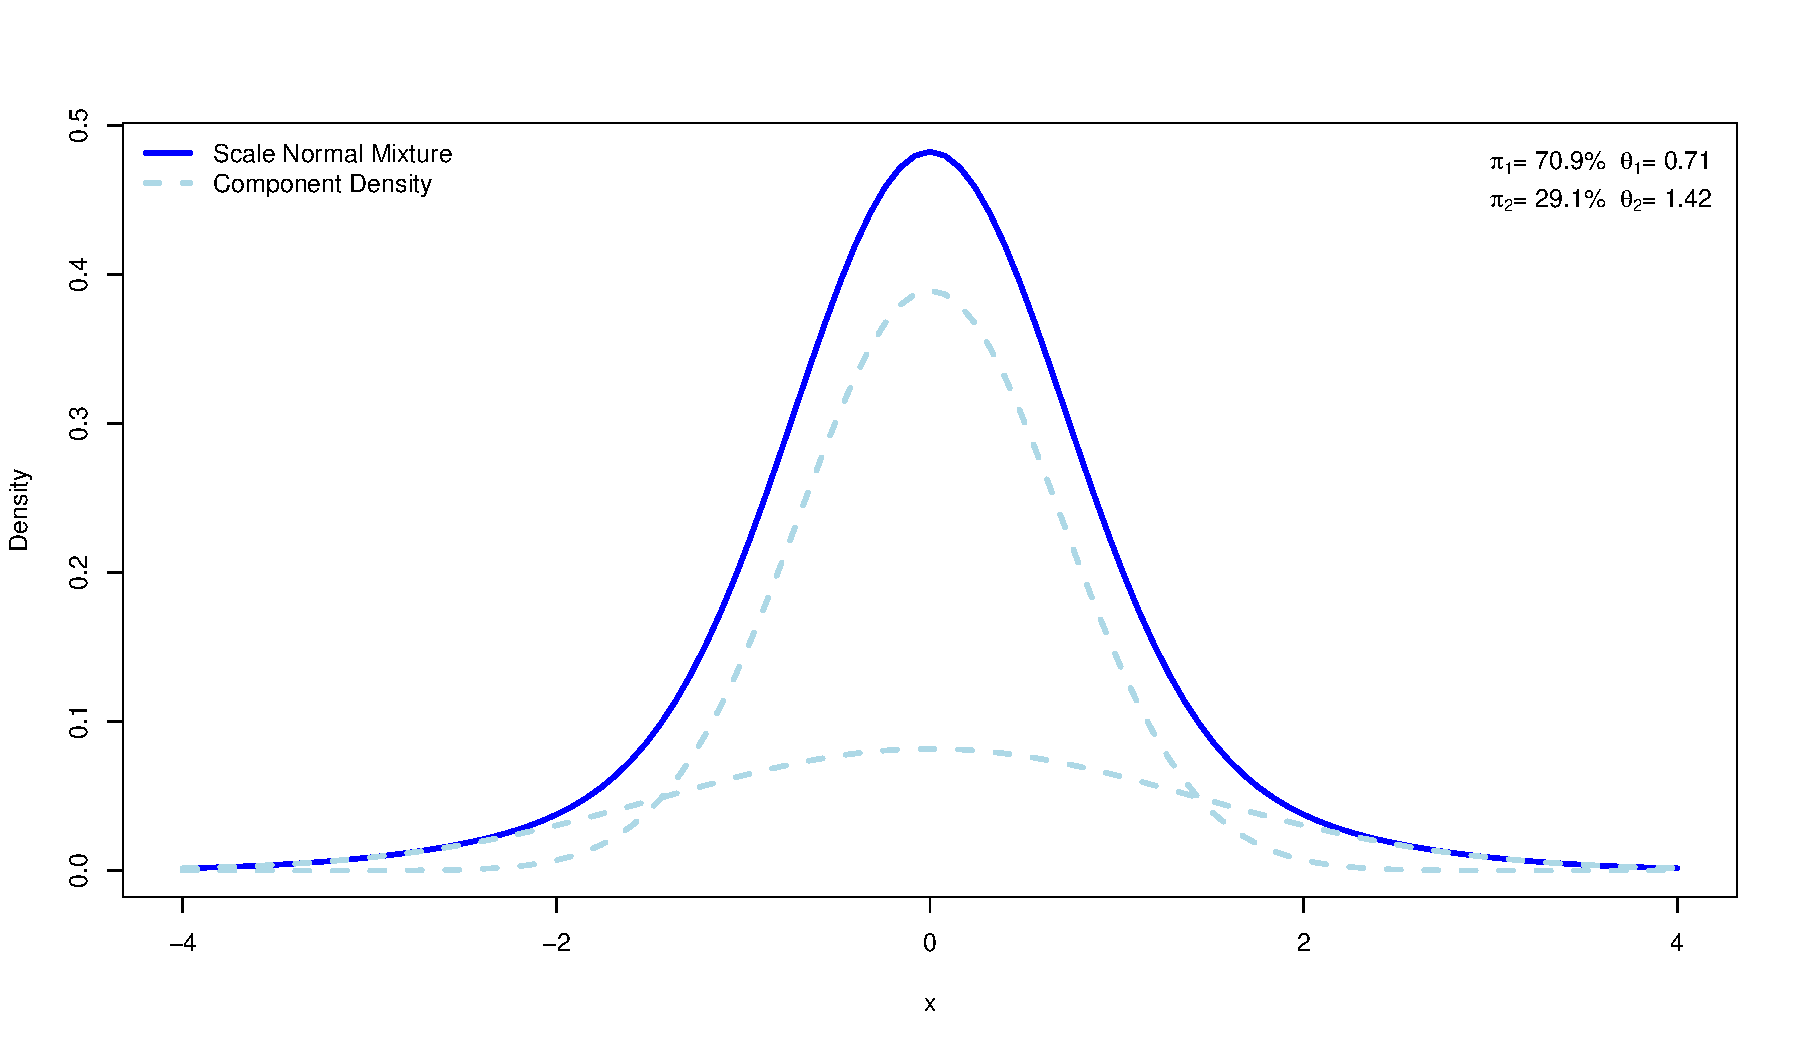
\includegraphics[scale = 0.35]{spComp.pdf}
}

\section{Conclusion}
\frame{
    \frametitle{Conclusion}
    \begin{itemize}
    \item A flexible frame work for GARCH modelling while preserving
      the theoretical advantage of the normal distribution.
    \item Further understand the source of volatility.
    \end{itemize}
}

\frame{
   \frametitle{Further Development}
   \begin{itemize}
   \item Extend to GARCH(p, q).
   \item Incorporate Skewness parameter in the model.
   \item Formal Tests.
   \end{itemize}
}
\frame{
    Thank you!!!!!!!!!!
}
\end{document}
